\section{Software Architectures}
Software architecture is the fundamental structure of a software system. Software architectures \textit{``represents the design decisions related to overall system structure and behavior. Architecture helps stakeholders understand and analyze how the system will achieve essential qualities such as modifiability, availability, and security''}~\citep{sei_software_architecture}.

Each architecture has its pros and cons. There are different types of software architectures adopted or sometimes introduced in order to solve certain issues. The most important ones that are necessary to be understood for this report are monolithic and microservices architectures.

\subsection{Monolithic Architecture}
Monolithic architecture is a traditional software development design paradigm where an application is built as a single, unified unit. All the components of the system are tightly coupled and dependent on each other. The monolithic architecture is simple, easier to design, develop and test and usually have easier deployment process as compared to some other architectures.

\subsection{Microservice Architecture}
Microservice architecture is a type of distributed system architecture and a software design in which a system is built as a collection of small, independent, and loosely coupled services. Each service is designed to keep in mind the Single-responsibility principle and hence has a specific function, operates independently and communicates with other services typically using HTTP or messaging queues. Distributed system architectures are easier to scale, flexible, autonomous and more resilient than other architectures, especially monolithic. 

\begin{figure}[H]
    \centering
    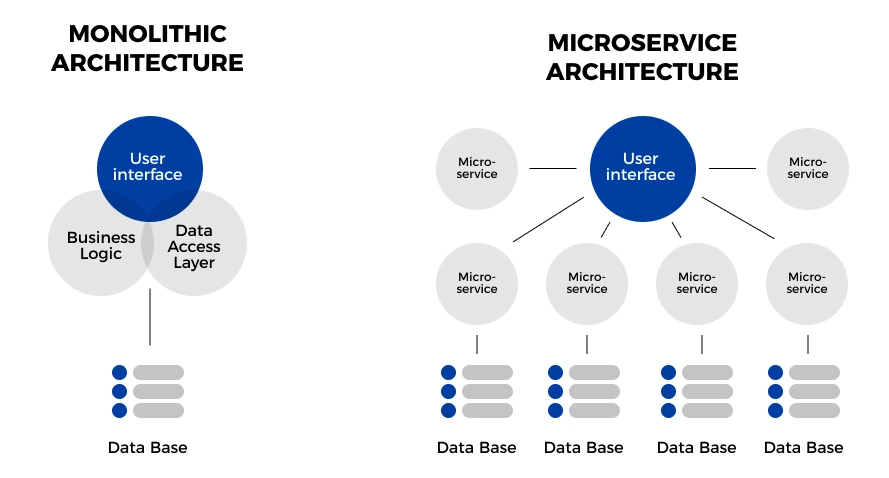
\includegraphics[width=0.7\textwidth]{figures/monolithic_microservices.png}
    \caption[Different between Monolithic \& Microservices Architecture]{Different between Monolithic \& Microservices Architecture\par (adapted from~\cite{atlassian_microservices_vs_monolith})}
	\label{fig_background_monolithic_microservices}
\end{figure}

\subsection{Spring Petclinic}\label{java_spring_petclinic}
Spring petclinic\footnote{\url{https://spring-petclinic.github.io/}} is a Java Spring framework based application that demonstrates best practices for building Java Spring applications. It was originally built using the monolithic architecture\footnote{\url{https://github.com/spring-projects/spring-petclinic}}, and then later on, the application system was split into independent services to demonstrate the best practices for Java Spring-based microservices\footnote{\url{https://github.com/spring-petclinic/spring-petclinic-microservices}}, Spring Boot, and Spring Cloud. The microservices-based Petclinic project is a good candidate for the case study since it is actively maintained and it’s widely used in the developer community for learning microservices best practices.

\begin{figure}[H]
    \centering
    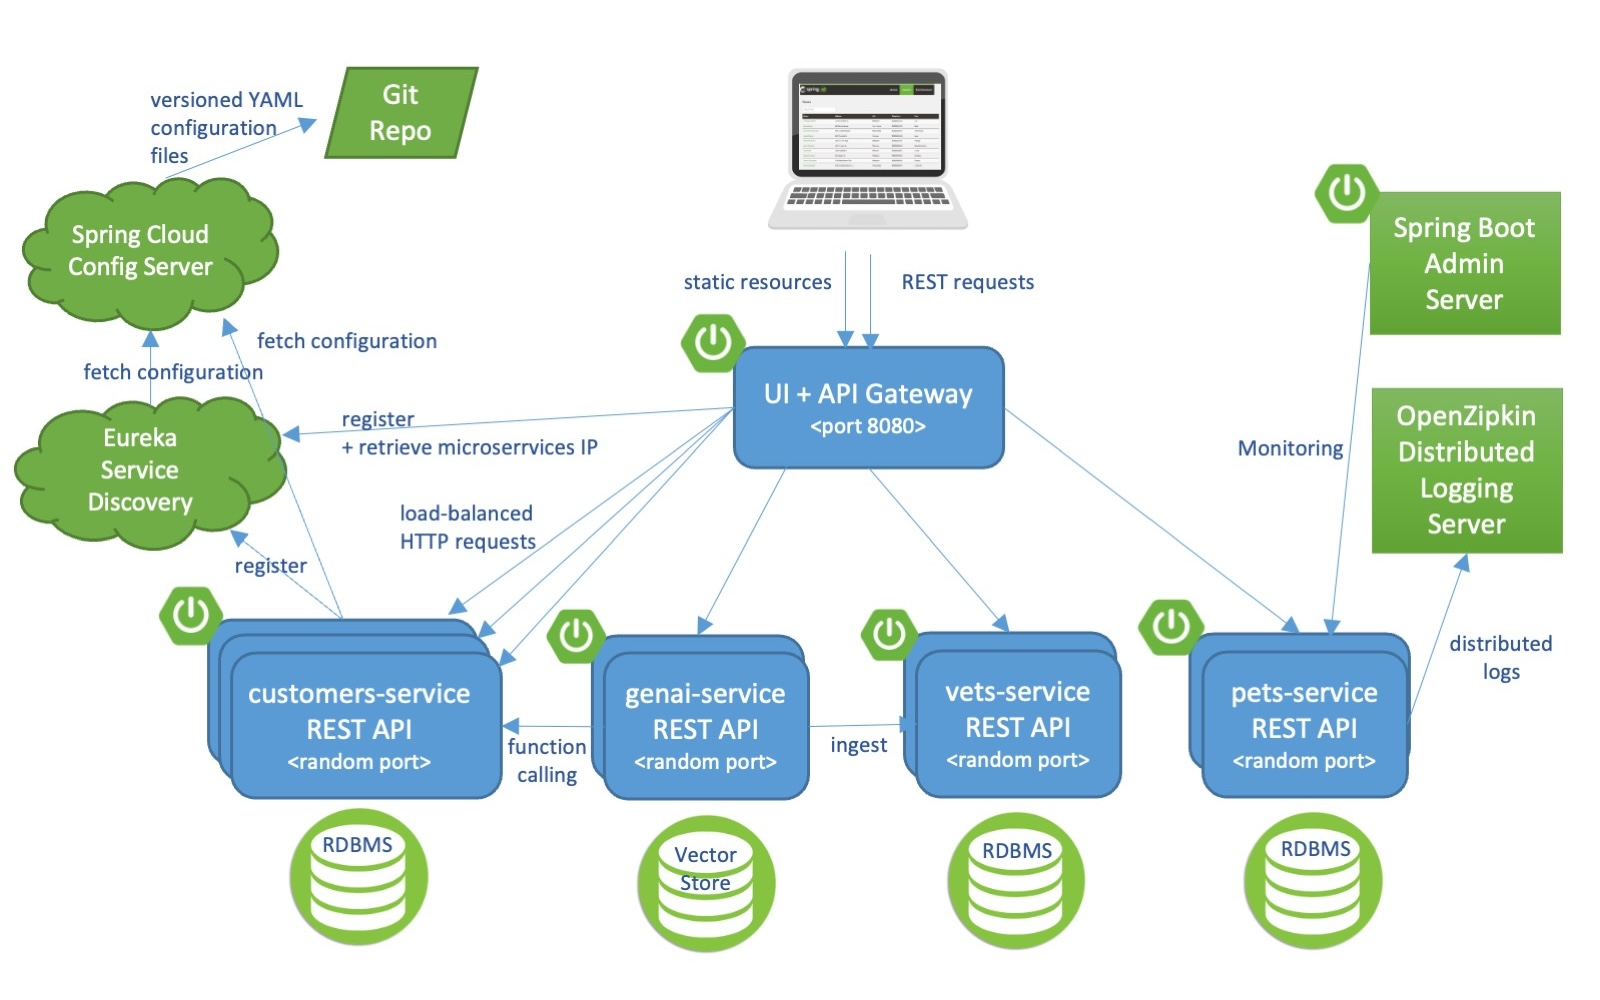
\includegraphics[width=1\textwidth]{figures/spring_petclinic_ms_architecture.jpg}
    \caption[Architecture diagram of the Spring Petclinic Microservices]{Architecture diagram of the Spring Petclinic Microservices\par (adapted from~\cite{SpringPetClinicMicroservices})}
	\label{fig_spring_petClinic_microservices}
\end{figure}

